% ============================================================
%  Demo for the "terminal" Beamer theme.
%  Compile with XeLaTeX or LuaLaTeX (twice, for the frame count).
%  On Overleaf: Menu > Settings > Compiler > XeLaTeX.
% ============================================================
\documentclass[aspectratio=169,10pt]{beamer}
\usetheme{terminal}            % options: nosectionpages, noprogressbar
\usepackage[brazil]{babel}
\usepackage{amsmath,amssymb}
\usepackage{booktabs}
\usepackage{appendixnumberbeamer} % backup slides don't count in [nn/NN]
\usepackage{pgfplots}
\pgfplotsset{compat=1.18}
\usepackage{ragged2e}
\usetikzlibrary{arrows.meta,positioning}
% !TeX program = xelatex

% ---------- theme settings ----------
\terminalfootprefix{demo}               % footline: "demo :: <short title>"
\terminalwindow{Método de Euler - agora vai}               % label in the title window bar
\terminalshell{%                        % fake shell session on the title page
  \$ make talk\\
  > compiling slides ............. ok\\
  > checking the coffee .......... ok}

\title[Método de Euler]{Método de Euler}
\subtitle{Analítico e numérico}
\author{[Joao Victor]}
\institute{[Instituto Federal do Amazonas]}
\date{\today}

\begin{document}

\begin{frame}[plain,noframenumbering]
  \titlepage
\end{frame}

\begin{frame}{Agenda}
\begin{tbox}{> ls talk/}
\small
\begin{tabular}{@{}l@{\quad}l@{}}
01 & Interpretação Geométrica \\
02 & Método de Euler - Passo simples \\
03 & Método de Euler Aperfeiçoado (RK2) \\
\end{tabular}
\end{tbox}
\end{frame}

% ============================================================
\section{Definição}

	\begin{frame}{Interpretação Geométrica}
		\justifying
		Dada uma equação diferencial $\dfrac{dy}{dx}=f(x,y)$ com condição de 
		contorno $y=y_{n}$ quando $x=x_{n}$: \\
		
		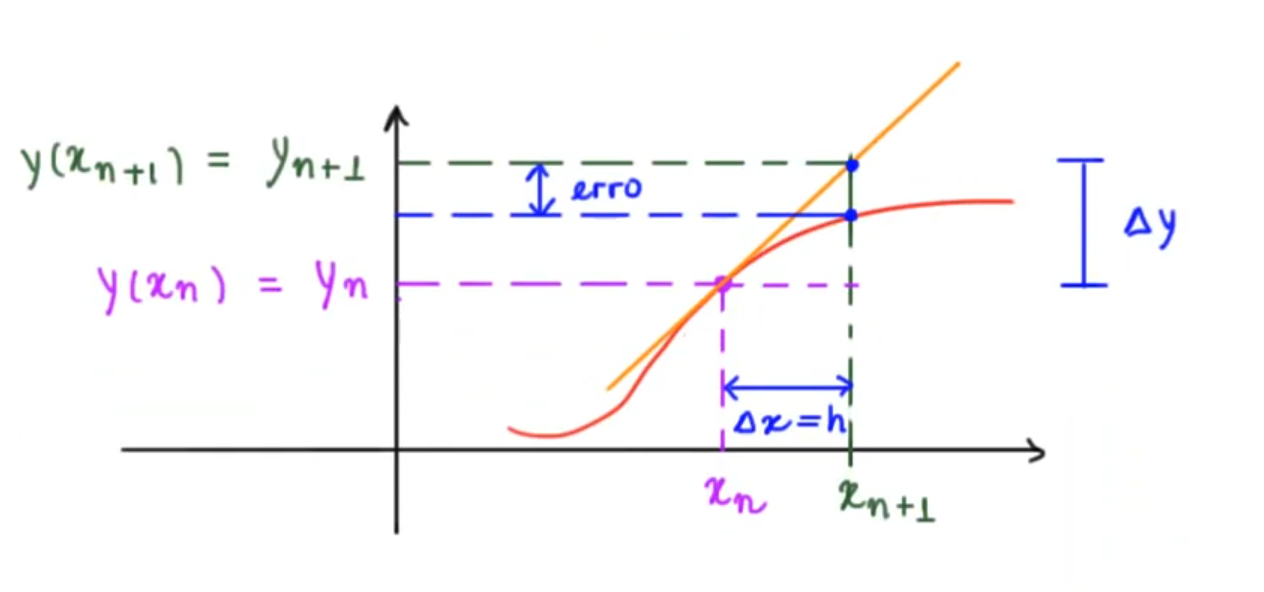
\includegraphics[scale=0.3]{imagens/euler.png}
	\end{frame}
	
	\begin{frame}{Aplicação}
		\justifying
		Aplique a formulação de Euler e estime o valor de $y(2,1)$ da EDO $xy'=3x-y$ com condição inicial $y(2)=2$ e passo $h=0,1$
	\end{frame}
	
	\begin{frame}{Aplicação 2}
		\justifying
		Aplique o método de Euler em $y'-y=2te^{2t}$ para $y(0)=1$ e estime o valor de $y(1)$, aplicando passo $h=0.5$
	\end{frame}

% ============================================================
\section{Método de Euler Aperfeiçoado (RK2)}

	\begin{frame}{Definição}
		\justifying
		Dado um problema de valor inicial (PVI) ${dy}/{dx}=f(x,y)$ e $y(x_{0})=x_{0}$ no método 
		em questão, vamos obter o valor da solução da EDO aplicada em outros pontos por meio de: \\
		
		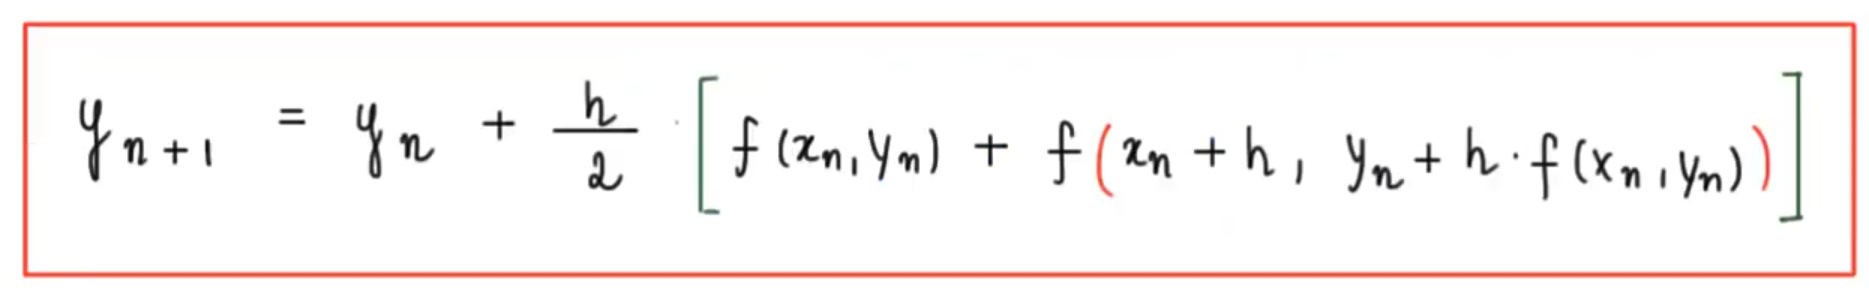
\includegraphics[scale=0.2]{imagens/euler2.png}
	\end{frame}
	
	\begin{frame}{Aplicação}
		\justifying
		Dado o PVI: $y'= \dfrac{2y}{x+1}+(x+1)^{3}$ e $y(0)=3$, obtenha $y(1)$ com $h=0,5$
		aplicando o \\ Método de Euler Aperfeiçoado. 
		
		%16,84
	\end{frame}
\end{document}
